\documentclass[a4paper,titlepage,10pt]{article}

\usepackage[T1]{fontenc}
\usepackage[utf8]{inputenc}
\usepackage{polski}

\usepackage{enumerate}
\usepackage{amssymb}
\usepackage{amsmath}
\usepackage[pdftex]{graphicx}
\usepackage{tikz}
\usepackage[colorlinks=true,linkcolor=blue]{hyperref}
\usepackage{anysize}

\usepackage[a4paper, top=2.5cm, bottom=2.5cm, left=2cm, right=2cm]{geometry}
\linespread{1.3}

\title{\huge Symulacja układu planetarnego na GPU\\ przy użyciu CUDA i OpenGL\\\small Dokumentacja biznesowa}
\author{Daniel Kłobuszewski\and Jakub Kotur}

\begin{document}
	\maketitle
	
	\marginsize{1cm}{1cm}{2.5cm}{2.5cm}

	\begin{figure}[h]
	\centering
\begin{tabular}{|p{.1\textwidth}|p{.04\textwidth}|p{.1\textwidth}|p{.1\textwidth}|p{.206\textwidth}|p{.1\textwidth}|}
	\hline
	\multicolumn{6}{|l|}{Metryka dokumentu} \\
	\hline
	Projekt & \multicolumn{2}{l|}{Symulacja układu planetarnego na GPU } &
	Firma & \multicolumn{2}{l|}{Politechnika Warszawska} \\
	&  \multicolumn{2}{l|}{przy użyciu CUDA i OpenGL} & &  \multicolumn{2}{l|}{} \\
	\hline
	Nazwa & \multicolumn{5}{l|}{Dokumentacja techniczna} \\
	\hline
	Temat & \multicolumn{5}{l|}{Specyfikacja techniczna projektu} \\
	\hline
	Autor & \multicolumn{5}{l|}{Daniel Kłobuszewski, Jakub Kotur} \\
	\hline
	Plik & \multicolumn{5}{l|}{tech.pdf} \\
	\hline
	Nr wersji & 06 & Status & Finalny & Data\par sporządzenia & 2010-10-09 \\
	\hline
	Streszczenie & \multicolumn{5}{p{11cm}|}{Celem dokumentu jest zdefiniowanie
		technicznych wymagań Projektu.} \\
	\hline
	Zatwierdził & \multicolumn{3}{l|}{ } &
	Data ostatniej\par modyfikacji & 2010-10-12 \\
	\hline
\end{tabular}

	\label{tab:metric}
\end{figure}



	\begin{figure}[h]
	\centering

\begin{tabular}{|p{.075\textwidth}|p{.1\textwidth}|p{.2\textwidth}|p{.522\textwidth}|}
	\hline
	\multicolumn{4}{|l|}{Historia zmian dokumentu} \\
	\hline
	Wersja & Data & Kto & Opis \\
	\hline
	0.1 & 2011-01-02 & Jakub Kotur &
	Określenie podstawowej struktury dokumentu \\
	\hline
	0.2 & 2011-01-04 & Jakub Kotur &
	Dodanie opisów dziłania oraz zmian \\
	\hline
	1.0 & 2011-01-04 & Daniel Kłobuszewski &
	Poprawki ortograficzne i stylistyczne \\
	\hline
\end{tabular}

	\label{tab:hist}
\end{figure}


	\marginsize{2cm}{2cm}{2.5cm}{2.5cm}

	\section{Wstęp}\label{sec:wstep}
	
	\paragraph{}



\begin{figure}[h]
	\centering
	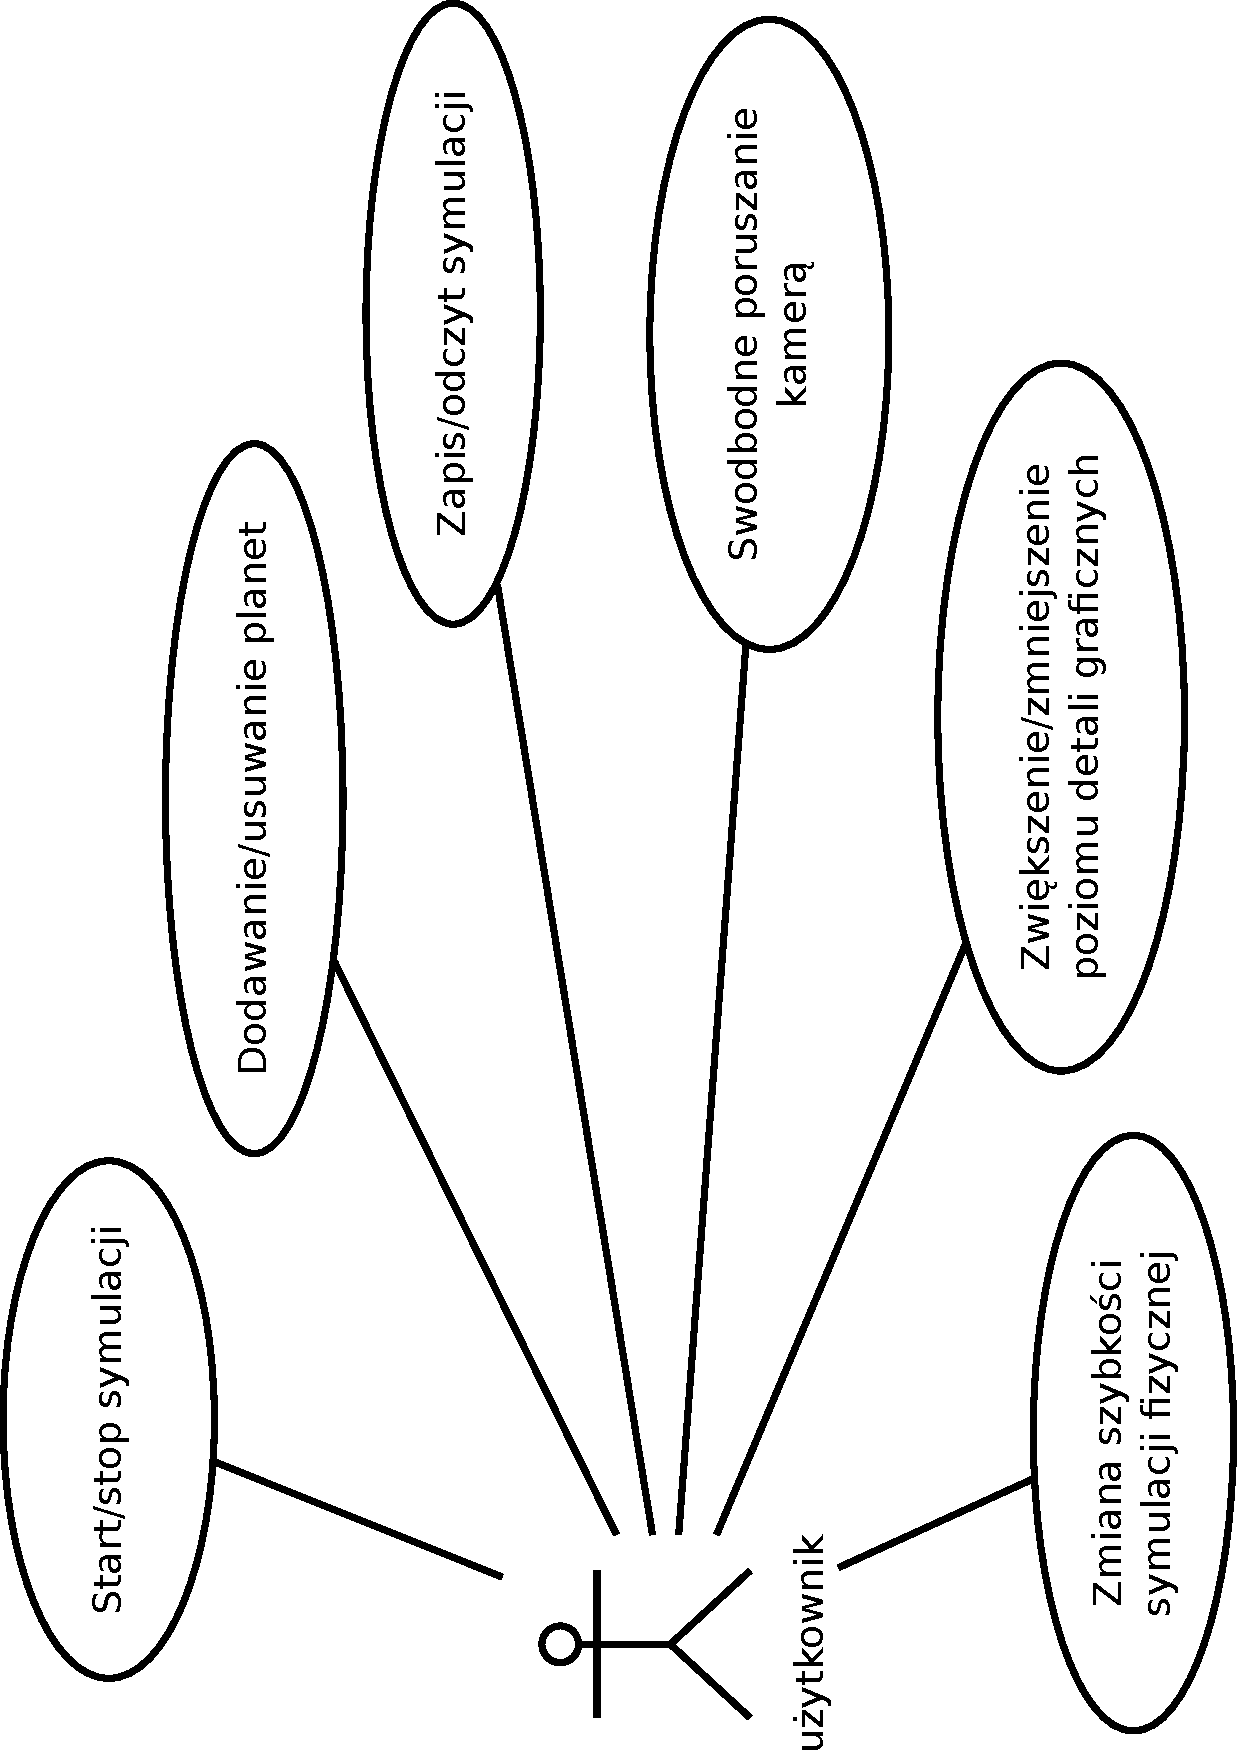
\includegraphics[width=0.7\textwidth,angle=-90]{use-case.pdf}
	\caption{Diagram przypadków użycia}
	\label{fig:use-case}
\end{figure}

\end{document}

